\documentclass[a4paper]{article}

\def\npart {III}
\def\nterm {Michaelmas}
\def\nyear {2016}
\def\nlecturer {J. A. Ross}
\def\ncourse {Differential Geometry}
\def\nlectures {MWF.11}

% Imports
\ifx \nextra \undefined
  \usepackage[pdftex,
    hidelinks,
    pdfauthor={Dexter Chua},
    pdfsubject={Cambridge Maths Notes: Part \npart\ - \ncourse},
    pdftitle={Part \npart\ - \ncourse},
  pdfkeywords={Cambridge Mathematics Maths Math \npart\ \nterm\ \nyear\ \ncourse}]{hyperref}
  \title{Part \npart\ - \ncourse}
\else
  \usepackage[pdftex,
    hidelinks,
    pdfauthor={Dexter Chua},
    pdfsubject={Cambridge Maths Notes: Part \npart\ - \ncourse\ (\nextra)},
    pdftitle={Part \npart\ - \ncourse\ (\nextra)},
  pdfkeywords={Cambridge Mathematics Maths Math \npart\ \nterm\ \nyear\ \ncourse\ \nextra}]{hyperref}

  \title{Part \npart\ - \ncourse \\ {\Large \nextra}}
\fi

\author{Lectured by \nlecturer \\\small Notes taken by Dexter Chua}
\date{\nterm\ \nyear}

\usepackage{alltt}
\usepackage{amsfonts}
\usepackage{amsmath}
\usepackage{amssymb}
\usepackage{amsthm}
\usepackage{booktabs}
\usepackage{caption}
\usepackage{enumitem}
\usepackage{fancyhdr}
\usepackage{graphicx}
\usepackage{mathtools}
\usepackage{microtype}
\usepackage{multirow}
\usepackage{pdflscape}
\usepackage{pgfplots}
\usepackage{siunitx}
\usepackage{tabularx}
\usepackage{tikz}
\usepackage{tkz-euclide}
\usepackage[normalem]{ulem}
\usepackage[all]{xy}

\pgfplotsset{compat=1.12}

\pagestyle{fancyplain}
\lhead{\emph{\nouppercase{\leftmark}}}
\ifx \nextra \undefined
  \rhead{
    \ifnum\thepage=1
    \else
      \npart\ \ncourse
    \fi}
\else
  \rhead{
    \ifnum\thepage=1
    \else
      \npart\ \ncourse\ (\nextra)
    \fi}
\fi
\usetikzlibrary{arrows}
\usetikzlibrary{decorations.markings}
\usetikzlibrary{decorations.pathmorphing}
\usetikzlibrary{positioning}
\usetikzlibrary{fadings}
\usetikzlibrary{intersections}
\usetikzlibrary{cd}

\newcommand*{\Cdot}{\raisebox{-0.25ex}{\scalebox{1.5}{$\cdot$}}}
\newcommand {\pd}[2][ ]{
  \ifx #1 { }
    \frac{\partial}{\partial #2}
  \else
    \frac{\partial^{#1}}{\partial #2^{#1}}
  \fi
}

% Theorems
\theoremstyle{definition}
\newtheorem*{aim}{Aim}
\newtheorem*{axiom}{Axiom}
\newtheorem*{claim}{Claim}
\newtheorem*{cor}{Corollary}
\newtheorem*{defi}{Definition}
\newtheorem*{eg}{Example}
\newtheorem*{fact}{Fact}
\newtheorem*{law}{Law}
\newtheorem*{lemma}{Lemma}
\newtheorem*{notation}{Notation}
\newtheorem*{prop}{Proposition}
\newtheorem*{thm}{Theorem}

\renewcommand{\labelitemi}{--}
\renewcommand{\labelitemii}{$\circ$}
\renewcommand{\labelenumi}{(\roman{*})}

\let\stdsection\section
\renewcommand\section{\newpage\stdsection}

% Strike through
\def\st{\bgroup \ULdepth=-.55ex \ULset}

% Maths symbols
\newcommand{\bra}{\langle}
\newcommand{\ket}{\rangle}

\newcommand{\N}{\mathbb{N}}
\newcommand{\Z}{\mathbb{Z}}
\newcommand{\Q}{\mathbb{Q}}
\renewcommand{\H}{\mathbb{H}}
\newcommand{\R}{\mathbb{R}}
\newcommand{\C}{\mathbb{C}}
\newcommand{\Prob}{\mathbb{P}}
\renewcommand{\P}{\mathbb{P}}
\newcommand{\E}{\mathbb{E}}
\newcommand{\F}{\mathbb{F}}
\newcommand{\cU}{\mathcal{U}}
\newcommand{\RP}{\mathbb{RP}}
\newcommand{\CP}{\mathbb{CP}}

\newcommand{\ph}{\,\cdot\,}

\DeclareMathOperator{\sech}{sech}
\DeclareMathOperator{\cosech}{cosech}
\DeclareMathOperator{\cosec}{cosec}

\DeclareMathOperator{\covol}{covol}
\DeclareMathOperator{\vol}{vol}

\let\Im\relax
\let\Re\relax
\DeclareMathOperator{\Im}{Im}
\DeclareMathOperator{\Re}{Re}
\DeclareMathOperator{\im}{im}
\DeclareMathOperator{\image}{image}
\DeclareMathOperator{\Ann}{Ann}

\DeclareMathOperator*{\res}{res}
\DeclareMathOperator{\Res}{Res}
\DeclareMathOperator{\Ind}{Ind}

\DeclareMathOperator{\tr}{tr}
\DeclareMathOperator{\diag}{diag}
\DeclareMathOperator{\rank}{rank}
\DeclareMathOperator{\card}{card}
\DeclareMathOperator{\spn}{span}
\DeclareMathOperator{\adj}{adj}

\DeclareMathOperator{\erf}{erf}
\DeclareMathOperator{\erfc}{erfc}

\DeclareMathOperator{\ord}{ord}
\DeclareMathOperator{\Sym}{Sym}

\DeclareMathOperator{\sgn}{sgn}
\DeclareMathOperator{\orb}{orb}
\DeclareMathOperator{\stab}{stab}
\DeclareMathOperator{\ccl}{ccl}

\DeclareMathOperator{\lcm}{lcm}
\DeclareMathOperator{\hcf}{hcf}

\DeclareMathOperator{\Int}{Int}
\DeclareMathOperator{\id}{id}

\DeclareMathOperator{\betaD}{beta}
\DeclareMathOperator{\gammaD}{gamma}
\DeclareMathOperator{\Poisson}{Poisson}
\DeclareMathOperator{\binomial}{binomial}
\DeclareMathOperator{\multinomial}{multinomial}
\DeclareMathOperator{\Bernoulli}{Bernoulli}
\DeclareMathOperator{\like}{like}

\DeclareMathOperator{\var}{var}
\DeclareMathOperator{\cov}{cov}
\DeclareMathOperator{\bias}{bias}
\DeclareMathOperator{\mse}{mse}
\DeclareMathOperator{\corr}{corr}

\DeclareMathOperator{\otp}{otp}
\DeclareMathOperator{\dom}{dom}

\DeclareMathOperator{\Root}{Root}
\DeclareMathOperator{\supp}{supp}
\DeclareMathOperator{\rel}{rel}
\DeclareMathOperator{\Hom}{Hom}
\DeclareMathOperator{\Aut}{Aut}
\DeclareMathOperator{\Gal}{Gal}
\DeclareMathOperator{\Mat}{Mat}
\DeclareMathOperator{\End}{End}
\DeclareMathOperator{\Char}{char}
\DeclareMathOperator{\ev}{ev}
\DeclareMathOperator{\St}{St}
\DeclareMathOperator{\Lk}{Lk}
\DeclareMathOperator{\disc}{disc}
\DeclareMathOperator{\Isom}{Isom}
\DeclareMathOperator{\length}{length}
\DeclareMathOperator{\energy}{energy}
\DeclareMathOperator{\area}{area}
\DeclareMathOperator{\Syl}{Syl}
\DeclareMathOperator{\cl}{cl}
\DeclareMathOperator{\fix}{fix}

\newcommand{\GL}{\mathrm{GL}}
\newcommand{\SL}{\mathrm{SL}}
\newcommand{\PGL}{\mathrm{PGL}}
\newcommand{\PSL}{\mathrm{PSL}}
\newcommand{\PSU}{\mathrm{PSU}}
\newcommand{\Or}{\mathrm{O}}
\newcommand{\SO}{\mathrm{SO}}
\newcommand{\U}{\mathrm{U}}
\newcommand{\SU}{\mathrm{SU}}

\renewcommand{\d}{\mathrm{d}}
\newcommand{\D}{\mathrm{D}}

\tikzset{->/.style = {decoration={markings,
                                  mark=at position 1 with {\arrow[scale=2]{latex'}}},
                      postaction={decorate}}}
\tikzset{<-/.style = {decoration={markings,
                                  mark=at position 0 with {\arrowreversed[scale=2]{latex'}}},
                      postaction={decorate}}}
\tikzset{<->/.style = {decoration={markings,
                                   mark=at position 0 with {\arrowreversed[scale=2]{latex'}},
                                   mark=at position 1 with {\arrow[scale=2]{latex'}}},
                       postaction={decorate}}}
\tikzset{->-/.style = {decoration={markings,
                                   mark=at position #1 with {\arrow[scale=2]{latex'}}},
                       postaction={decorate}}}
\tikzset{-<-/.style = {decoration={markings,
                                   mark=at position #1 with {\arrowreversed[scale=2]{latex'}}},
                       postaction={decorate}}}

\tikzset{circ/.style = {fill, circle, inner sep = 0, minimum size = 3}}
\tikzset{mstate/.style={circle, draw, blue, text=black, minimum width=0.7cm}}

\definecolor{mblue}{rgb}{0.2, 0.3, 0.8}
\definecolor{morange}{rgb}{1, 0.5, 0}
\definecolor{mgreen}{rgb}{0.1, 0.4, 0.2}
\definecolor{mred}{rgb}{0.5, 0, 0}

\def\drawcirculararc(#1,#2)(#3,#4)(#5,#6){%
    \pgfmathsetmacro\cA{(#1*#1+#2*#2-#3*#3-#4*#4)/2}%
    \pgfmathsetmacro\cB{(#1*#1+#2*#2-#5*#5-#6*#6)/2}%
    \pgfmathsetmacro\cy{(\cB*(#1-#3)-\cA*(#1-#5))/%
                        ((#2-#6)*(#1-#3)-(#2-#4)*(#1-#5))}%
    \pgfmathsetmacro\cx{(\cA-\cy*(#2-#4))/(#1-#3)}%
    \pgfmathsetmacro\cr{sqrt((#1-\cx)*(#1-\cx)+(#2-\cy)*(#2-\cy))}%
    \pgfmathsetmacro\cA{atan2(#2-\cy,#1-\cx)}%
    \pgfmathsetmacro\cB{atan2(#6-\cy,#5-\cx)}%
    \pgfmathparse{\cB<\cA}%
    \ifnum\pgfmathresult=1
        \pgfmathsetmacro\cB{\cB+360}%
    \fi
    \draw (#1,#2) arc (\cA:\cB:\cr);%
}
\newcommand\getCoord[3]{\newdimen{#1}\newdimen{#2}\pgfextractx{#1}{\pgfpointanchor{#3}{center}}\pgfextracty{#2}{\pgfpointanchor{#3}{center}}}

\def\Xint#1{\mathchoice
   {\XXint\displaystyle\textstyle{#1}}%
   {\XXint\textstyle\scriptstyle{#1}}%
   {\XXint\scriptstyle\scriptscriptstyle{#1}}%
   {\XXint\scriptscriptstyle\scriptscriptstyle{#1}}%
   \!\int}
\def\XXint#1#2#3{{\setbox0=\hbox{$#1{#2#3}{\int}$}
     \vcenter{\hbox{$#2#3$}}\kern-.5\wd0}}
\def\ddashint{\Xint=}
\def\dashint{\Xint-}


\begin{document}
\maketitle
{\small
\setlength{\parindent}{0em}
\setlength{\parskip}{1em}
This course is intended as an introduction to modern differential geometry. It can be taken with a view to further studies in Geometry and Topology and should also be suitable as a supplementary course if your main interests are for instance in Analysis or Mathematical Physics. A tentative syllabus is as follows.

\begin{itemize}[label={$\bullet$}]
 \item \emph{Local Analysis and Differential Manifolds.} Definition and examples of manifolds, smooth maps. Tangent vectors and vector fields, tangent bundle. Geometric consequences of the implicit function theorem, submanifolds. Lie Groups.
 \item \emph{Vector Bundles.} Structure group. The example of Hopf bundle. Bundle morphisms and automorphisms. Exterior algebra of differential forms. Tensors. Symplectic forms. Orientability of manifolds. Partitions of unity and integration on manifolds, Stokes Theorem; de Rham cohomology. Lie derivative of tensors. Connections on vector bundles and covariant derivatives: covariant exterior derivative, curvature. Bianchi identity.

 \item \emph{Riemannian Geometry.} Connections on the tangent bundle, torsion. Bianchi's identities for torsion free connections. Riemannian metrics, Levi-Civita connection, Christoffel symbols, geodesics. Riemannian curvature tensor and its symmetries, second Bianchi identity, sectional curvatures.
\end{itemize}

\subsubsection*{Pre-requisites}
An essential pre-requisite is a working knowledge of linear algebra (including bilinear forms) and multivariate calculus (e.g. differentiation and Taylor's theorem in several variables). Exposure to some of the ideas of classical differential geometry might also be useful.
}
\tableofcontents

\section{Manifolds}
Intuitively, a manifold is something that locally looks like (an open subset of) $\R^n$. On an open set of $\R^n$, we know what it means for something to be differentiable, twice differentiable, or smooth. Since these are local properties, this allows us to talk about whether a function to or from a manifold is differentiable, twice differentiable or smooth.

\begin{defi}[Chart]\index{chart}
  A chart $(U, \varphi)$ on a set $M$ is a bijection $\varphi: U \to \varphi(U) \subseteq \R^n$, where $U \subseteq M$ and $\varphi(U)$ is open.

  A chart $(U, \varphi)$ is \emph{centered at $p$}\index{center} for $p \in U$ if $\varphi(p) = 0$.
\end{defi}

\begin{center}
  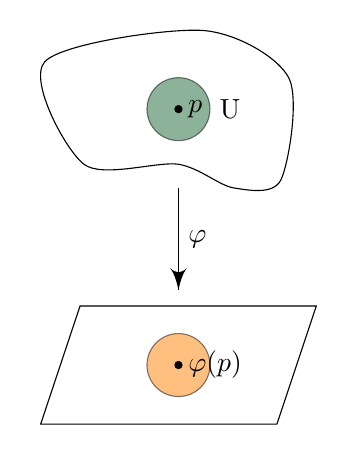
\begin{tikzpicture}
    \draw plot [smooth cycle] coordinates {(-1.2, -0.7) (0, -0.7) (0.7, -1) (1.3, -0.9) (1.4, 0.4) (0.3, 1) (-1.7, 0.6)};

    \draw [fill=mgreen, opacity=0.5] circle [radius=0.4];
    \node [right] {$p$};
    \node [circ] {};
    \node at (0.4, 0) [right] {U};

    \begin{scope}[shift={(-1.75, -4)}]
      \draw (0, 0) -- (3, 0) -- (3.5, 1.5) -- (0.5, 1.5) -- cycle;

      \draw (1.75, 0.75) [fill=morange, opacity=0.5] circle [radius=0.4];
      \node at (1.75, 0.75) [right] {$\varphi(p)$};
      \node at (1.75, 0.75) [circ] {};
    \end{scope}

    \draw [->] (0, -1) -- +(0, -1.3) node [pos=0.5, right] {$\varphi$};
  \end{tikzpicture}
\end{center}

\begin{defi}[Smooth function]\index{smooth function}\index{$C^\infty$}
  Let $(U, \varphi)$ be a chart on $M$, and $f: M \to \R$, we say $f$ is \emph{smooth} or $C^\infty$ at $p \in U$ if $f \circ \varphi^{-1}: \varphi(U) \to \R$ is smooth at $\varphi(p)$ in the usual sense.
  \[
    \begin{tikzcd}
      \R^n \supseteq \varphi(U) \ar[r, "\varphi^{-1}"] & U \ar[r, "f"] & \R
    \end{tikzcd}
  \]
\end{defi}
We can define all other notions such as continuity, differentiability, twice differentiability etc. similarly.

This definition has a problem that some points might not be in the chart, and we don't know how to determine if a function is, say, smooth at the point. The solution is easy --- we just take many charts that together cover $M$. However, we have the problem that a function might be smooth at a point relative to some chart, but not relative to some other chart. The solution is to require the charts to be compatible in some sense.

\begin{defi}[Atlas]\index{atlas}
  An \emph{atlas} on a set $M$ is a collection of charts $\{(U_\alpha, \varphi_\alpha)\}$ on $M$ such that
  \begin{enumerate}
    \item $M = \bigcup_{\alpha} U_\alpha$.
    \item For all $\alpha, \beta$, we have $\varphi_\alpha(U_\alpha \cap U_\beta)$ is open in $\R^n$, and the transition function
      \[
        \varphi_\alpha \circ \varphi_\beta^{-1}: \varphi_\beta(U_\alpha \cap U_\beta) \to \varphi_\alpha(U_\alpha \cap U_\beta)
      \]
      is smooth (in the usual set).
  \end{enumerate}
\end{defi}

\begin{lemma}
  If $(U_\alpha, \varphi_\alpha)$ and $(U_\beta, \varphi_\beta)$ are charts in some atlas, and $f: M \to \R$, then $f \circ \varphi_\alpha^{-1}$ is smooth at $\varphi_\alpha(p)$ if and only if $f \circ \varphi_\beta^{-1}$ is smooth at $\varphi_\beta (p)$ for all $p \in U_\alpha \cap U_\beta$.
\end{lemma}

\begin{proof}
  We have
  \[
    f \circ \varphi_\beta^{-1} = f \circ \varphi_\alpha^{-1} \circ (\varphi_\alpha \circ \varphi_\beta^{-1}).
  \]
\end{proof}

\begin{eg}
  Consider the sphere
  \[
    S^2 = \{(x_1, x_2, x_2): \sum x_i^2 = 1\} \subseteq \R^3.
  \]
  We let
  \[
    U_1^+ = S^2 \cap \{x_1 > 0\},\quad U_1^- = S^2 \cap \{x_1 < 0\}, \cdots
  \]
  We then let
  \begin{align*}
    \varphi_1^+: U_1^+ &\to \R^2\\
    (x_1, x_2, x_3) &\mapsto (x_2, x_3).
  \end{align*}
  It is easy to show that gives a bijection to the open disk in $\R^3$. We similarly define the other $\phi_i^{\pm}$. These then give us an atlas of $S^2$.
\end{eg}

\begin{defi}[Equivalent atlases]\index{equivalent atlases}\index{atlas, equivalence}
  Two atlases $\mathcal{A}_1$ and $\mathcal{A}_2$ are \emph{equivalent} if $\mathcal{A}_1 \cup \mathcal{A}_2$ is an atlas.
\end{defi}

\begin{defi}[Differentiable structure]\index{differentiable structure}
  A \emph{differentiable structure} on $M$ is a choice of equivalence class of atlases.
\end{defi}

We want to define a manifold to be a set with a differentiable structure. However, we still have the problem of giving it a topology. It turns out the smooth structure already gives us a topology.

\begin{ex}
  An atlas determines an topology on $M$ be saying $V \subseteq M$ is open iff $\varphi(U \cap V)$ is open in $\R^n$ for all charts $(U, \varphi)$ in the atlas. Equivalent atlases give the same topology.
\end{ex}

We now get to the definition of a manifold.

\begin{defi}[Manifold]\index{manifold}
  A \emph{manifold} is a set $M$ with a choice of differentiable structure whose topology is
  \begin{enumerate}
    \item Hausdorff\index{Hausdorff}, ie. for all $x, y \in M$, there are open neighbourhoods $U_x, U_y \subseteq M$ with $x \in U_x, y \in U_y$ and $U_x \cap U_y = \emptyset$.
    \item Second countable\index{second countable}, ie. there exists a countable collection $(U_n)_{n \in \N}$ of open sets in $M$ such that for all $V \subseteq M$ open, and $p \in V$, there is some $n$ such that $p \in U_n \subseteq V$.
  \end{enumerate}
\end{defi}
These requirements are there just to make sure we do not have pathological spaces. For example, the Hausdorff condition excludes the line with two origins from being a manifold, and the second countability condition excludes the long line. We will not use the second countability condition much.

Note that we will often refer to a manifold simply as $M$, where the differentiable structure is understood from context. By a chart on $M$, we mean one in some atlas in the equivalence class of atlases.

Say $\varphi: U \to \varphi(U) \subseteq \R^n$ is a chart of $M$. We think of $\varphi$ as $\varphi = (x_1, \cdots, x_n)$, with $x_i: U \to \R$. We call the $x_i$ the \emph{local coordinates}\index{local coordinates}. By abuse of notation, if $f: M \to \R$, we confuse $f|_U$ and $f \circ \varphi^{-1}: \varphi(U) \to \R$. So we write $f(x_1, \cdots, x_n)$ to mean $f(p)$, where $\varphi(p) = (x_1, \cdots, x_n) \in \varphi(U)$.
\[
  \begin{tikzcd}
    U \ar[r, hook, "\iota"] \ar[d, "\varphi"] & M \ar[r, "f"] & \R\\
    \varphi(U) \ar[rru, "f|_U"']
  \end{tikzcd}
\]
Of course, we can similarly define $C^0, C^1, C^2, \cdots$ manifolds, or analytic manifolds. We can also model manifolds on other spaces, eg. $\C^n$, where we get complex manifolds, or on infinite-dimensional spaces.

\begin{eg}\leavevmode
  \begin{enumerate}
    \item Generalizing the example of the sphere, the $n$-dimensional sphere $S^n = \{(x_0, \cdots, x_n) \in \R^{n + 1}: \sum x_i^2 = 1\}$ is a manifold.
    \item If $M$ is open in $\R^n$, then the inclusion map $\varphi: M \to \R^n$ given by $\varphi(p) = p$ is a chart forming an atlas. So $M$ is a manifold. In particular, $\R^n$ is a manifold, with its ``standard'' differentiable structure. We will always assume $\R^n$ is given this structure, unless otherwise specified.
    \item $M(n, n)$, the set of all $n \times n$ matrices is also a manifold, by the usual bijection with $\R^{n^2}$. Then $\GL_n \subseteq M(n, n)$ is open, and thus also a manifold.
    \item The set $\RP^n$, the set of one-dimensional subspaces of $\R^{n + 1}$ is a manifold. We can define charts as follows: we let $U_i$ to be the lines spanned by a vector of the form $(v_0, v_1, \cdots, v_{i - 1}, 1, v_{i + 1}, \cdots, v_n) \in \R^n$.

      We define the map $\varphi_i: U_i \to \R^n \cong \{\mathbf{x} \in \R^{n + 1}: x_i = 1\}$ that sends $\varphi(L) = (v_0, \cdots, 1, \cdots, v_n)$, where $L$ is spanned by $(v_0, \cdots, 1, \cdots, v_n)$. It is an easy exercise to show that this defines a chart.
  \end{enumerate}
\end{eg}

Note that when we defined a chart, we talked about charts as maps $U \to \R^n$. We did not mention whether $n$ is fixed, or whether it is allowed to vary. It turns out it cannot vary, as long as the space is connected.

\begin{lemma}
  Let $M$ be a manifold, and $\varphi_1: U_1 \to \R^n$ and $\varphi_2: U_2 \to \R^m$ be charts. If $U_1 \cap U_2 \not= \emptyset$, then $n = m$.
\end{lemma}

\begin{proof}
  We have $\varphi_1 \varphi_2^{-1}: \varphi_2(U_1 \cap U_2) \to \varphi_1(U_1 \cap U_2)$ is a smooth map with inverse $\varphi_2 \varphi_1^{-1}$. So $D(\varphi_1 \varphi_2^{-1})(\varphi(p)): \R^m \to \R^n$ is a linear isomorphism, whenever $p \in U_1 \cap U_2$. So $n = m$.
\end{proof}

\begin{defi}[Dimension]\index{dimension}
  If $p \in M$, we say $M$ has \emph{dimension} $n$ at $p$ if for one (thus all) charts $\varphi: U \to \R^m$ with $p \in U$, we have $m = n$. We say $M$ has dimension $n$ if it has dimension $n$ at all points.
\end{defi}

\section{Smooth functions and derivatives}
From now on, $M$ and $N$ will be manifolds.

\begin{defi}[Smooth function]\index{smooth function}
  A function $f: M \to N$ is \emph{smooth at a point $p \in M$} if there are charts $(U, \varphi)$ for $M$ and $(V, \zeta)$ for for $N$ with $p \in U$ and $f(p) \in V$ such that $\zeta \circ f \circ \varphi^{-1}: \varphi(U) \to \zeta(V)$ is smooth at $\varphi(p)$.

  A function is \emph{smooth} if it is smooth at all points $p \in M$.

  A \term{diffeomorphism} is a smooth $F$ with a smooth inverse.

  We write $C^\infty(M, N)$ \index{$C^\infty(M, N)$} for the space of smooth maps $F: M \to N$. We write $C^\infty(M)$\index{$C^\infty(M)$} for $C^\infty(M, \R)$, and this has the additional structure of an algebra, ie. vector space with multiplication.
\end{defi}

Equivalently, $f$ is smooth at $p$ if $\zeta \circ F \circ \varphi^{-1}$ is smooth at $\varphi(p)$ for \emph{any} such charts $(U, \varphi)$ and $(V, \zeta)$.

\begin{eg}
  Let $\varphi: U \to \R^n$ be a chart. Then $\varphi: U \to \varphi(U)$ is a diffeomorphism.
\end{eg}

\begin{defi}[Curve]\index{curve}
  A \emph{curve} is a smooth map $I \to M$, where $I$ is a non-empty open interval.
\end{defi}

To discuss derivatives, we first look at the case where $U \subseteq \R^n$ is open. Suppose $f: U \to \R$ is smooth. If $p \in U$ and $v \in \R^n$, recall that the \term{directional derivative} is defined by
\[
  Df|_p(v) = \lim_{t \to 0} \frac{f(p + t\mathbf{v}) - f(p)}{t}.
\]
If $\mathbf{v} = \mathbf{e}_i = (0, \cdots, 1, 0, \cdots, 0)$, then we write
\[
  Df|_p (\mathbf{e}_i) = \left.\frac{\partial f}{\partial x_i}\right|_p.
\]
Also, we know $Df|_p: \R^n \to \R$ is a linear map (by definition of smooth).

Note that here $p$ and $\mathbf{v}$ are both vectors, but they play different roles --- $p$ is an element in the domain $U$, while $\mathbf{v}$ is an arbitrary vector in $\R^n$. Even if $\mathbf{v}$ is enormous, by taking a small enough $t$, we find that $p + t\mathbf{v}$ will eventually be inside $U$.

If we have a general manifold, we can still talk about the $p$. However, we don't have anything that plays the role of a vector. Our first goal is to define the tangent space to a manifold that captures where the ``directions'' live.

An obvious way to do so would be to use a curve. Suppose $\gamma: I \to M$ is a curve, with $\gamma(0) = p \in U \subseteq M$, and $f: U \to \R$ is smooth. We can then take the derivative of $f$ along $\gamma$ as before. We let
\[
  X(f) = \left.\frac{\d}{\d t}\right|_{t = 0} f(\gamma(t)).
\]
It is an exercise to see that $X: C^\infty(U) \to \R$ is a linear map, and it satisfies the \term{Leibnitz rule}
\[
  X(fg) = f(p) X(g) + g(p) X(f).
\]
We denote $X$ by $\dot{\gamma}(0)$. We might think of defining the tangent space as curves up to some equivalence relation, but if we do this, there is no obvious vector space on it. However, if we define a tangent vector as a linear map satisfying the Leibnitz rule, then it has an automatic, obvious vector space structure.
\begin{defi}[Derivation]\index{derivation}
  A \emph{derivation} on an open subset $U \subseteq M$ at $p \in U$ is a linear map $X: C^\infty(U) \to \R$ satisfying the Leibnitz rule
  \[
    X(fg) = f(p) X(g) + g(p) X(f).
  \]
\end{defi}

\begin{defi}[Tangent space]\index{tangent space}
  Let $p \in U \subseteq M$, where $U$ is open. The \emph{tangent space} of $M$ at $p$ is the vector space
  \[
    T_p(M) = \{\text{derivations on $U$ at $p$}\}.
  \]
  The subscript $p$ tells us the point at which we are taking the tangent space.
\end{defi}
We will later show that this does not depend on $U$. It is easy to see that if $\gamma: i \to M$ is a curve with $\gamma(0) = p$, then $\dot{\gamma}(0) = T_p(M)$. We will also later show that all derivations do come from some path, which is less trivial.

\begin{eg}
  Let $U \subseteq \R^n$ be open, and let $p \in U$. Let $D_{e_i, q} \in T_q \R^n$ be
  \[
    D_{e_i, q} = \left.\frac{\partial f}{\partial x_i}\right|_q.
  \]
\end{eg}

\begin{lemma}
  $\{D_{e_1, q}, \cdots, D_{e_n, q}\}$ is a basis of $T_q \R^n$. So these are all the derivations.
\end{lemma}

The idea of the proof is to show that a derivation can only depend on the first order derivatives of a function, and all possibilities will be covered by the $D_{e_i, q}$.

\begin{proof}
  Independence is clear as
  \[
    D_{e_i, q}(x_j) = \frac{\partial x_j}{\partial x_i} = \delta_{ij}.
  \]
  We need to show spanning. For notational convenience, we wlog $q = 0$. Let $X \in T_0 \R^n$.

  We first show that if $g \in C^\infty(U)$ is the constant function $g = 1$, then $X(g) = 0$. Indeed, we have
  \[
    X(g) = X(g^2) = g(0) X(g) + X(g) g(0) + 2 X(g).
  \]
  Thus, if $h$ is any constant function, say, $c$, then $X(h) = X(cg) = c X(g)$. So the derivative of any constant function vanishes.

  In general, let $f \in C^\infty(U)$. By Taylor's theorem, we have
  \[
    f(x_1, \cdots, x_n) = f(0) + \sum \frac{\partial f}{\partial x_i} x_i + \varepsilon,
  \]
  where $\varepsilon$ is a sum of terms of the form $x_i x_j h$ with $h \in C^\infty(U)$.

  We set $\lambda_i = X(x_i) \in \R$. We first claim that $X(\varepsilon) = 0$. Indeed, we have
  \[
    X (x_i x_j h) = x_i|_{0} X(x_j h) + (x_jh)(0) X(x_i) = 0.
  \]
  So we have
  \[
    X(f) = \sum \lambda_i \left.\frac{\partial f}{\partial x_i}\right|_0.
  \]
  So we have
  \[
    X = \sum \lambda_i D_{e_i, q}.
  \]
\end{proof}

\begin{defi}[Derivative]\index{derivative}
  Suppose $F \in C^\infty(M, N)$, say $F(p) = q$. We define $\D F|_p: T_p M \to T_q N$ by
  \[
    \D F|_p(X)(g) = X(g \circ F)
  \]
  for $X \in T_pM$ and $g \in C^\infty(V)$ with $q \in V \subseteq N$.

  This is a linear map called the \emph{derivative} of $F$ at $p$.
\end{defi}

\begin{prop}[Chain rule]\index{chain rule}
  Let $M, N, P$ be manifolds, and $F \in C^\infty(M, N)$, $G \in C^\infty(N, P)$, and $p \in M, q \in F(p)$. Then we have
  \[
    \D(G \circ F)|_p = \D G|_q \circ \D F|_p.
  \]
\end{prop}

\begin{proof}
  We have
  \[
    (\D F|_p (X))(h) = \D F|_p(X) (h \circ G) = X(h \circ G \circ F) = \D (G \circ F)|_p (X).
  \]
\end{proof}

\begin{cor}
  If $F$ is a diffeomorphism, then $\D F|_p$ is a linear isomorphism, and $(\D F|_p)^{-1} = \D (F^{-1})|_{F(p)}$.
\end{cor}

We now go back to understanding what $T_pM$ is if $p \in M$. We let $p \in U$ where $(U, \varphi)$ be a chart. Then if $q = \varphi(p)$, then $D\varphi|_p: T_p M \to T_q \R^n$ is a linear isomorphism.

\begin{defi}[$\frac{\partial}{\partial x_i}$]\index{$\frac{\partial}{\partial x_i}$}
  Given a chart $\varphi: U \to \R^n$ with $\varphi = (x_1, \cdots, x_n)$, we define
  \[
    \left.\frac{\partial}{\partial x_i}\right|_p = (D \varphi|_p)^{-1} (D_{e_i, q}) \in T_p M.
  \]
\end{defi}
So $\left.\frac{\partial}{\partial x_1}\right|_p, \left.\frac{\partial}{\partial x_2}\right|_p, \cdots$ are a basis for $T_p M$.

Recall that if $f: U \to \R$ is smooth, we write $f(x_1, \cdots, x_n)$. Then we have
\[
  \left.\frac{\partial}{\partial x_i}\right|_p (f) = \left.\frac{\partial f}{\partial x_i}\right|_{\varphi(p)}.
\]
So we have a consistent notation.

Now how does this basis change when we change coordinates? Suppose we also have coordinates $y_1, \cdots, y_n$ near $p$ given by some other chart. We then have $\left.\frac{\partial}{\partial y_i}\right|_p \in T_p M$. So we have
\[
  \left.\frac{\partial}{\partial y_i}\right|_p = \sum_j \alpha_j \left.\frac{\partial}{\partial x_j}\right|_p
\]
for some $\alpha_j$. To figure out what they are, we apply them to the function $x_k$. So we have
\[
  \left.\frac{\partial x_k}{\partial y_i}\right|_p = \alpha_k.
\]
So we obtain
\[
  \frac{\partial}{\partial y_i} = \sum_j \frac{\partial x_j}{\partial y_i} \frac{\partial}{\partial x_j}.
\]
This is the usual change-of-coordinate formula!

Now recall that if $F \in C^\infty (M, N)$ with $F(p) = q$, then we obtain a linear map $\D F|_p: T_pM \to T_q N$ given by
\[
  \D F|_p(X)(g) = X(g \circ F)
\]
for $X \in T_p(M)$ and $g \in C^\infty (V, \R)$.

Now suppose $(U, \varphi)$ is a chart on $M$ containing $p$ with coordinates $x_1, \cdots, x_n$, and $(V, \zeta)$ is a chart on $N$ containing $q$ with coordaintes $y_1,\cdots, y_m$.

By abuse of notation, we confuse $F$ and $\zeta \circ F \circ \varphi^{-1}$. So we write $F = (F_1, \cdots, F_n)$ with $F_i = F_i(x_1, \cdots, x_n): U \to \R$.

As before, we have a basis
\begin{align*}
  \left.\frac{\partial}{\partial x_i}\right|_p, \cdots, \left.\frac{\partial}{\partial x_n}\right|_p&\quad\text{for}\quad T_pM,\\
  \left.\frac{\partial}{\partial y_i}\right|_q, \cdots, \left.\frac{\partial}{\partial y_m}\right|_q&\quad\text{for}\quad T_qN.
\end{align*}

\begin{lemma}
  We have
  \[
    \D F|_p \left(\left.\frac{\partial}{\partial x_i}\right|_p\right) = \sum_{j = 1}^n \frac{\partial F_j}{\partial x_i}(p) \left.\frac{\partial}{\partial y_j}\right|_p.
  \]
  In other words, $\D F|_p$ has matrix representation
  \[
    \left(\frac{\partial F_j}{\partial x_i}(p)\right)_{ij}.
  \]
\end{lemma}

\begin{proof}
  We let 
  \[
    \D F|_p \left(\left.\frac{\partial}{\partial x_i}\right|_p\right) = \sum_{j = 1}^n \lambda_j \left.\frac{\partial}{\partial y_j}\right|_p.
  \]
  for some $\lambda_i$. We apply this to the local function $y_k$ to obtain
  \begin{align*}
    \lambda_k &= \left(\sum \lambda_j \left.\frac{\partial}{\partial y_j}\right|_p\right)(y_k)\\
    &= \D F_p \left(\left.\frac{\partial}{\partial x_i}\right|_p\right)(y_k)\\
    &= \left.\frac{\partial}{\partial x_i}\right|_p (y_k \circ F) = \left.\frac{\partial}{\partial x_i}\right|_p(F_k) = \frac{\partial F_k}{\partial x_i}(p).
  \end{align*}
\end{proof}

\begin{eg}
  Let $f: C^\infty(U)$ where $U \subseteq M$ is an open set containing $p$. Then $\D f|_p: T_p M \to T_{f(p)} \R \cong \R$ is a linear map. So $\D f|_p$ is an element in the dual space $(T_pM)^*$, called the \term{differential} of $f$ at $p$, and is denoted $\d f|_p$.
\end{eg}

Recall that there is one thing we swept under the carpet --- to define the tangent space, we needed to pick an open set $U$. Ways to deal with this can be found in the example sheet, but there are two general approaches --- one is to talk about germs of functions, where we consider all open neighbourhoods, and identify two functions if they agree on some open neighbourhood of the point. The other way is to realize that we can ``extend'' any function on $U \subseteq M$ to a function on the whole of $M$, using bump functions.

In general, we want a function that looks like this:
% insert picture

\begin{lemma}
  Suppose $W \subseteq M$ is a coordinate chart with $p \in W$. then there is an open neighbourhood $V$ of $p$ such that $\bar{V} \subseteq W$ and an $X \in C^\infty(M, \R)$ such that $x = 1$ on $V$ and $W = 0$ on $M \setminus W$.
\end{lemma}

\begin{proof}
  Suppose we have coordiantes $x_1, \cdots, x_n$ on $W$. We wlog suppose these are defined for all $|x| < 3$.

  We define $\alpha, \beta, \gamma: \R \to \R$ by
  \[
    \alpha(t) =
    \begin{cases}
      e^{-t^{-2}} & t > 0\\
      0 & t \leq 0
    \end{cases}.
  \]
  \begin{center}
    \begin{tikzpicture}
      \draw [->] (-3, 0) -- (3, 0);
      \draw [->] (0, -0.5) -- (0, 3);
      \draw [thick, blue] (-3, 0) -- (0, 0);
      \draw [domain=0.01:3, thick, blue] plot [smooth] (\x, {2 * exp(- 1 / (\x * \x))});
    \end{tikzpicture}
  \end{center}
  We now let
  \[
    \beta(t) = \frac{\alpha(t)}{\alpha(t) + \alpha(1 - t)}.
  \]
  \begin{center}
    \begin{tikzpicture}[xscale=4]
      \draw [->] (0, 0) -- (1, 0);
      \draw [->] (0, -0.5) -- (0, 3);
      \draw [thick, blue] (0, 0) -- (0.01, 0);
      \draw [domain=0.01:0.99, thick, blue] plot [smooth] (\x, {2 * (exp(- 1 / (\x * \x)))/((exp(- 1 / (\x * \x))) + (exp(- 1 / ((1 - \x) * (1 - \x)))))});
    \end{tikzpicture}
  \end{center}
  Then we let
  \[
    \gamma(t) = \beta(t + 2)\beta(2 - t).
  \]
  \begin{center}
    \begin{tikzpicture}
      \draw [->] (-3, 0) -- (3, 0);
      \draw [->] (0, -0.5) -- (0, 3);
      \draw [thick, blue] (-1.01, 2) -- (1.01, 2);
      \draw [thick, blue] (-3, 0) -- (-1.99, 0);
      \draw [thick, blue] (1.99, 0) -- (3, 0);
      \draw [domain=-1.99:-1.01, thick, blue] plot [smooth] (\x, {2 * (exp(- 1 / ((2 + \x) * (2 + \x))))/((exp(- 1 / ((2 + \x) * (2 + \x)))) + (exp(- 1 / ((-1 - \x) * (-1 - \x)))))});
      \draw [domain=1.01:1.99, thick, blue] plot [smooth] (\x, {2 * (exp(- 1 / ((2 - \x) * (2 - \x))))/((exp(- 1 / ((2 - \x) * (2 - \x)))) + (exp(- 1 / ((-1 + \x) * (-1 + \x)))))});
    \end{tikzpicture}
  \end{center}
  Finally, we let
  \[
    X(x_1, \cdots, x_n) = \gamma(x_1) \cdots \gamma(x_n).
  \]
  on $W$. We let
  \[
    V = \{\mathbf{x}: |x_i| < 1\}.
  \]
  Extending $X$ to be identically $0$ on $M \setminus W$ to get the desired smooth function (up to some constant).
\end{proof}
\begin{lemma}
  Let $p \in W \subseteq U$ and $W, U$ open. Let $f_1, f_2 \in C^\infty(U)$ be such that $f_1 = f_2$ on $W$. Then if $X \in \Der_p(C^\infty(U))$, then we have $X(f_1) = X(f_2)$
\end{lemma}

\begin{proof}
  Set $h = f_1 - f_2$. We can wlog $W$ is a coordinate chart. We pick a bump function $\chi \in C^\infty(U)$ that vanishes outside $W$. Then $\chi h = 0$. Then we have
  \[
    0 = X(\chi h) = \chi(p) X(h) + h(p) X(\chi) = X(h) + 0 = X(f_1) - X(f_2).
  \]
\end{proof}

\section{Submanifolds}
You have a manifold, and a subset of it is a manifold, so you call it a submanifold. Except there are some subtleties here. There will be two kinds of submanifolds we can talk about, namely embedded submanifolds and immersed submanifold.

\begin{defi}[Embedded submanifold]\index{Embedded submanifold}
  Let $M$ be a manifold with $\dim M = n$, and $S$ be a submanifold of $M$. We say $S$ is an \emph{embedded manifold} if for all $p \in S$, there are coordinates $x_1, \cdots, x_n$ on some chart $U \subseteq M$ containing $p$ such that
  \[
    S \cap U = \{x_{k + 1} = x_{k + 2} = \cdots = x_n = 0\}.
  \]
  Such coordinates are known as \term{slice coordinates} for $S$.
\end{defi}

\begin{lemma}
  If $S$ is an embedded submanifold of $M$, then there exists a unique differential structure on $S$ such that the inclusion map $\iota: S \hookrightarrow M$ is smooth.
\end{lemma}

\begin{proof}
  Basically if $x_1, \cdots, x_n$ is a slice chart for $S$ in $M$, then $x_1,  \cdots, x_k$ will be coordinates on $S$.

  More precisely, let $\pi: \R^n \to \R^k$ be the projection map
  \[
    \pi(x_1, \cdots, x_n) = (x_1, \cdots, x_k).
  \]
  Given a slice chart $(U, \varphi)$ for $S$ in $M$, consider $\tilde{\varphi}: S \cap U \to \R^k$ by $\tilde{\varphi} = \pi \circ \varphi$. This is smooth and bijective, and is so a chart on $S$. These cover $S$ by assumption. So we only have to check that the transition functions are smooth.

  Given another slice chart $(V, \zeta)$ for $S$ in $M$, we let $\tilde{\zeta} = \pi \circ \zeta$, and check that
  \[
    \tilde{\zeta} \circ \tilde{\varphi}^{-1} = \pi \circ \zeta \circ \varphi^{-1} \circ j,
  \]
  where $j: \R^k \to \R^n$ is given by $j(x_1, \cdots, x_k) = (x_1, .., x_k, 0, \cdots, 0)$.

  We can also check easily that $\iota: S\to M$ is smooth, and this is the only differential structure with this property.
\end{proof}

\printindex
\end{document}
